\documentclass[tikz]{standalone}

\tikzset{
	source/.pic = {
		\draw (0.5, 0.7) -- ++(0, -0.2) --
		      ++(-0.5, 0) -- ++(0, 0.5) --
		      ++(-0.7, 0) -- ++(0, -2) --
		      ++(0.7, 0) -- ++(0, 0.5) --
		      ++(0.5, 0) -- ++(0, -0.2);
	},
	detector/.pic = {
		\draw [fill=gray] (-1, 1) rectangle (1, -1);
		\draw (-0.8, 1) -- ++(0, -2);
	},
	slab/.pic = {
		\draw [fill=gray!50] (-0.2, 2) rectangle (0.2, -2);
	},
	human/.pic = {
		\draw [fill=gray] (0, 0) 
		.. controls ++(180:-1) and ++(-90: 1) .. ( 2, 1)
		.. controls ++(-90:-1) and ++(180:-1) .. ( 0, 2)
		.. controls ++(180: 1) and ++(-90:-1) .. (-2, 1)
		.. controls ++(-90: 1) and ++(180: 1) .. ( 0, 0);
		\draw [fill=white] (0, 1.5) ellipse (0.8 and 1);
		\draw (-.1, 2.49) to [in=180, out=30] ++(0.1, 0.2) to [in=150, out=0] ++(0.1, -0.2);
		\path[thick, fill=white] (-.1, 2.48) to [in=180, out=30] ++(0.1, 0.2) to [in=150, out=0] ++(0.1, -0.2) --cycle;
	}
}

\usetikzlibrary{shapes.arrows}
\begin{document}
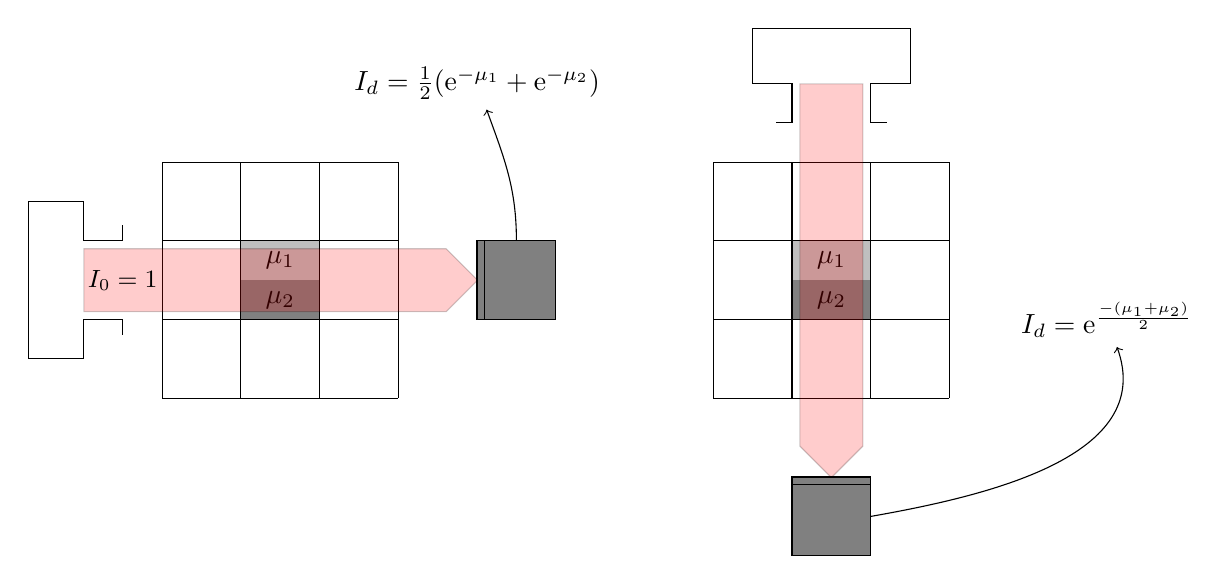
\begin{tikzpicture}
	\def\size{3}
	\fill [gray!50] (1, -1) rectangle (2, -1.5) node [midway, black] {\( \mu_1 \)};
	\fill [gray] (1, -1.5) rectangle (2, -2) node [midway, black] {\( \mu_2 \)};
	\foreach [count=\i] \x in {0,...,\size}
	{
		\draw  (\x, 0) -- ++(0, -\size);
	}
	\foreach [count=\j] \y in {0,...,-\size}
	{
		\draw (0, \y) -- ++(\size, 0);
	}
	\node[
		draw, fill=red, single arrow, opacity=0.2,
		minimum height=5cm, minimum width=8mm,
		single arrow head extend=0mm,
		anchor=west,
	] at (-1, -1.5) {};
	\pic at (-1, -1.5) {source};
	\node at (-0.5, -1.5) {\small \( I_0 = 1 \)};
	\pic[scale=0.5, local bounding box=detector] at (4.5, -1.5) {detector};
	\node (annot1) at (4, 1) {\( I_d = \frac{1}{2} (\mathrm{e}^{-\mu_1} + \mathrm{e}^{-\mu_2}) \)};
	\draw [->] (detector) to[out=90, in=-70] (annot1);
	\begin{scope}[shift={(7, 0)}]
		\fill [gray!50] (1, -1) rectangle (2, -1.5) node [midway, black] {\( \mu_1 \)};
		\fill [gray] (1, -1.5) rectangle (2, -2) node [midway, black] {\( \mu_2 \)};
		\foreach [count=\i] \x in {0,...,\size}
		{
			\draw  (\x, 0) -- ++(0, -\size);
		}
		\foreach [count=\j] \y in {0,...,-\size}
		{
			\draw (0, \y) -- ++(\size, 0);
		}
		\node[
			draw, fill=red, single arrow, opacity=0.2,
			minimum height=5cm, minimum width=8mm,
			single arrow head extend=0mm,
			anchor=west, rotate=-90,
		] at (1.5, 1) {};
		\pic [rotate=-90]  at (1.5, 1) {source};
		\pic[scale=0.5, local bounding box=detector, rotate=-90] at (1.5, -4.5) {detector};
	\node (annot1) at (5, -2) {\( I_d = \mathrm{e}^{\frac{-(\mu_1 + \mu_2)}{2}}\)};
		\draw [->] (detector.east) to[out=10, in=-70] (annot1);
	\end{scope}
\end{tikzpicture}
\end{document}
